\section{Results}
\subsection{Two-body system}
\begin{figure}[h]
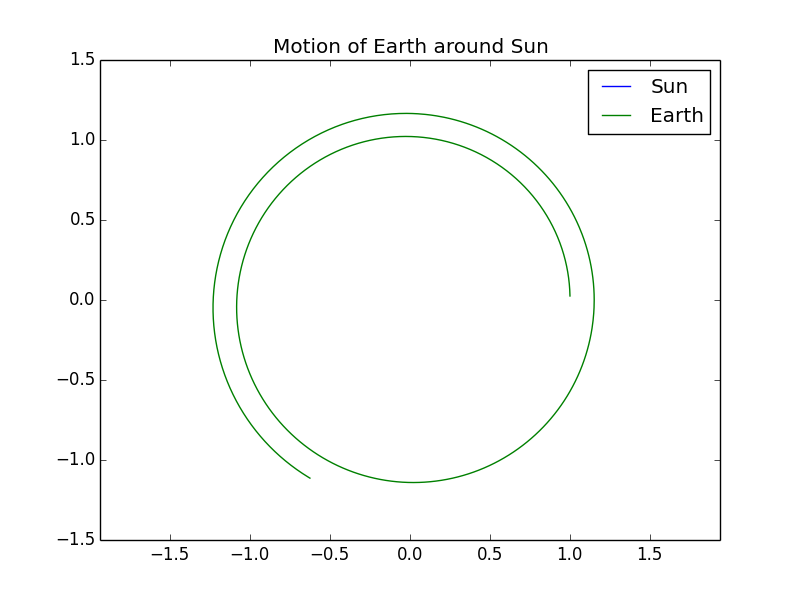
\includegraphics[scale=0.7]{figures/earth_sun_euler}
\caption{The plot shows the simulated orbit of the Earth around the Sun using the forward Euler integration method. The motion is simulated for two years, with $\Delta t = 0.002$ years.}
\end{figure}


\begin{figure}[h]
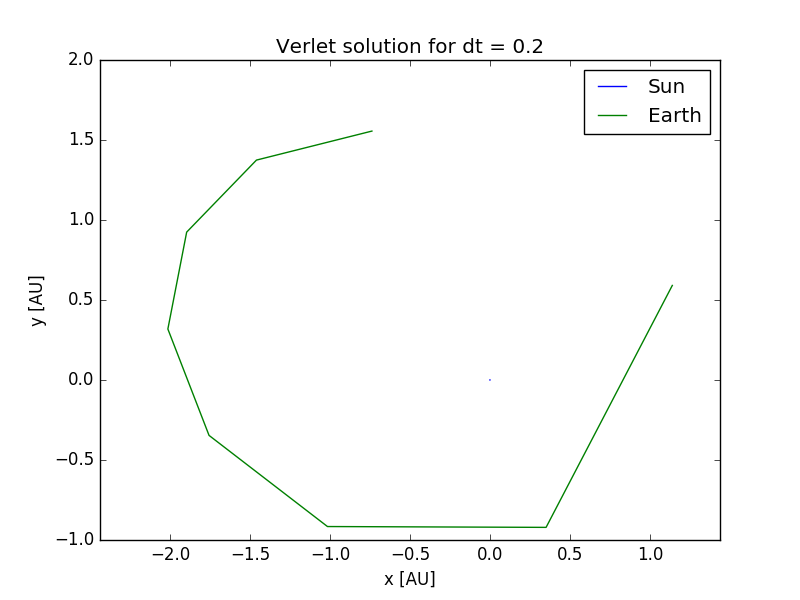
\includegraphics[scale=0.7]{figures/verlet_02}
\caption{The plot shows the simulated orbit of the Earth around the Sun using the velocity-Verlet integration method. The motion is simulated for two years, with $\Delta t = 0.2$ years}
\end{figure}

\begin{figure}[h]
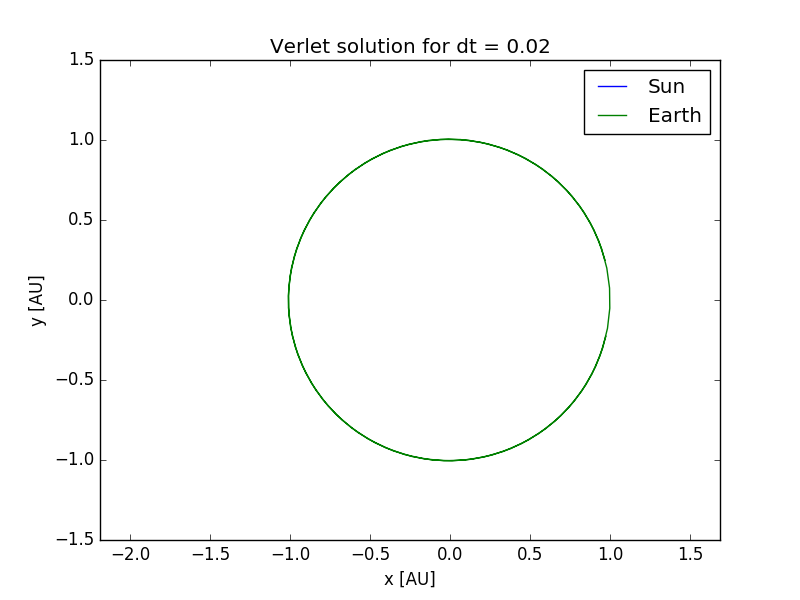
\includegraphics[scale=0.7]{figures/verlet_002}
\caption{The plot shows the simulated orbit of the Earth around the Sun using the velocity-Verlet integration method. The motion is simulated for two years, with $\Delta t = 0.02$ years}
\end{figure}



\begin{figure}[h]
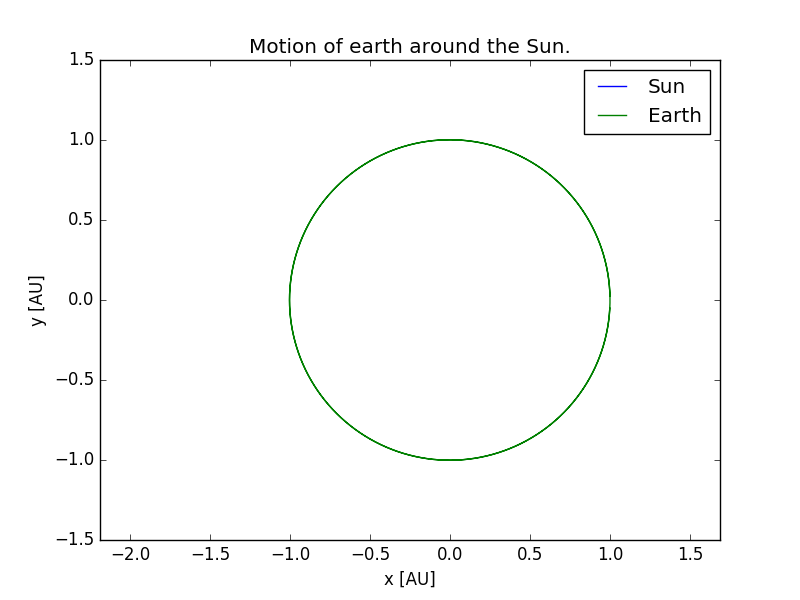
\includegraphics[scale=0.7]{figures/earth_sun_verlet}
\caption{The plot shows the simulated orbit of the Earth around the Sun using the velocity-Verlet integration method. The motion is simulated for two years, with $\Delta t = 0.002$ years.}
\end{figure}

The Euler method does not pass the tests for conservation of kinetic energy, potential energy and angular momentum for $\Delta t = 0.002$\ref{•}

\subsubsection{Escape velocity}\label{results:escape-velocity}
Using the model for the two-body system, a trial and error process of finding the escape velocity
for a planet with initial position 1AU away from the sun was performed. The calculations were
performed using the velocity Verlet method.
\begin{figure}[h]
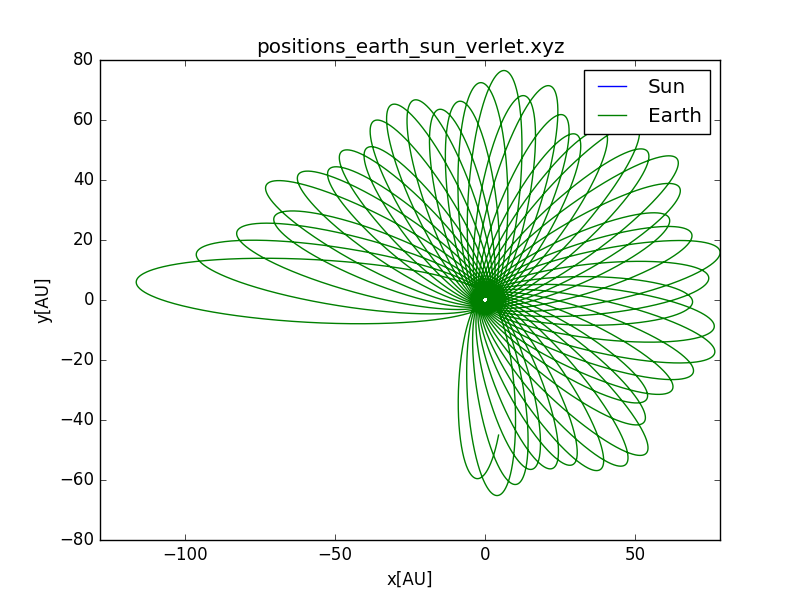
\includegraphics[width=\textwidth]{figures/escape_86}
\label{tab:comp-time}
\caption{The plot shows the position of a planet relative to the sun as a function of time when 
the planet has $v_{init} = 8.6\tfrac{AU}{yr}$}
\end{figure}
\begin{figure}[h]
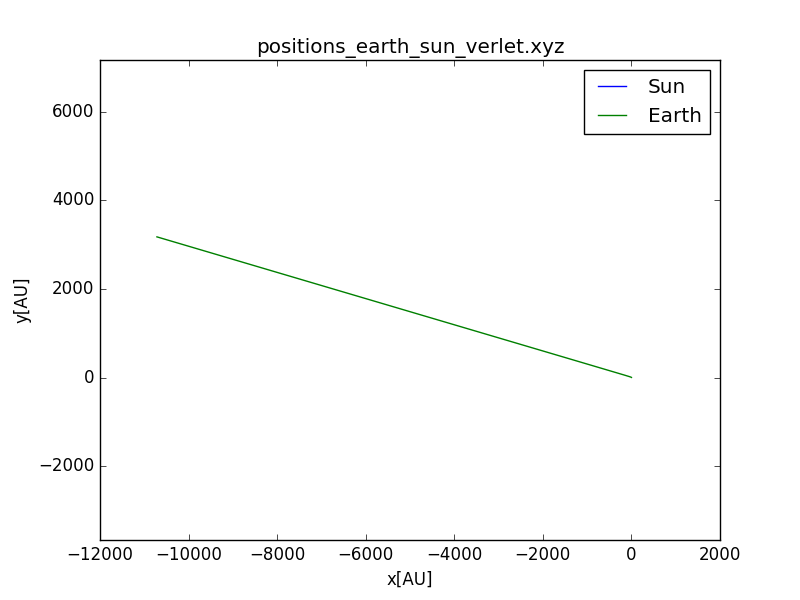
\includegraphics[width=\textwidth]{figures/escape_87}
\caption{The plot shows the position of a planet relative to the sun as a function of time when 
the planet has $v_{init} = 8.7\tfrac{AU}{yr}$}
\end{figure}

\begin{table}
\centering
\caption{Table of execution times for a final time of 10000 years}
\begin{tabular}{|l|l|}
\hline
\textbf{Method}  & \textbf{Time[s]} \\
\hline
Forward Euler   & 0.416121 \\
\hline
Velocity Verlet & 1.17558 \\
\hline
\end{tabular}
\end{table}

\subsection{Three-body system}
\begin{figure}[h]
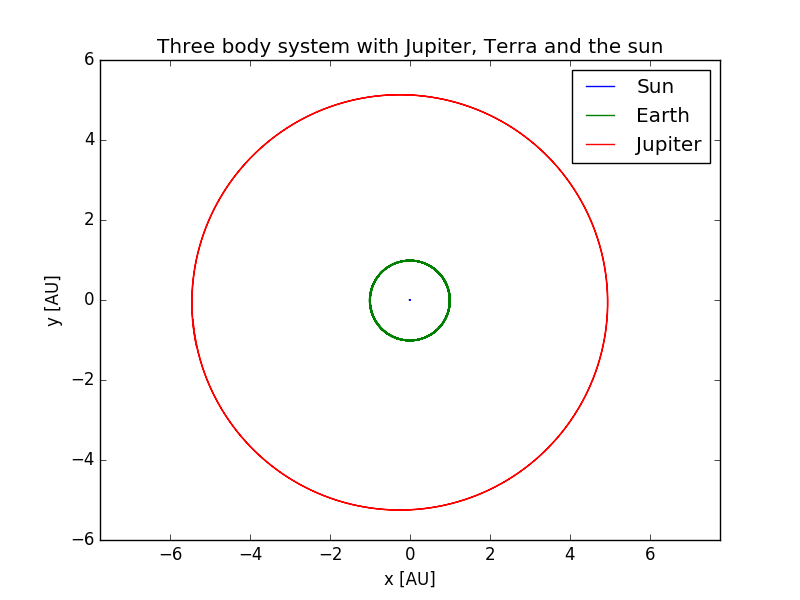
\includegraphics[scale=0.7]{figures/three_body}[h]
\caption{The plot shows the orbit of Earth and Jupiter around the barycentre }
\end{figure}

\subsection{Full solar system}
\begin{figure}[h]
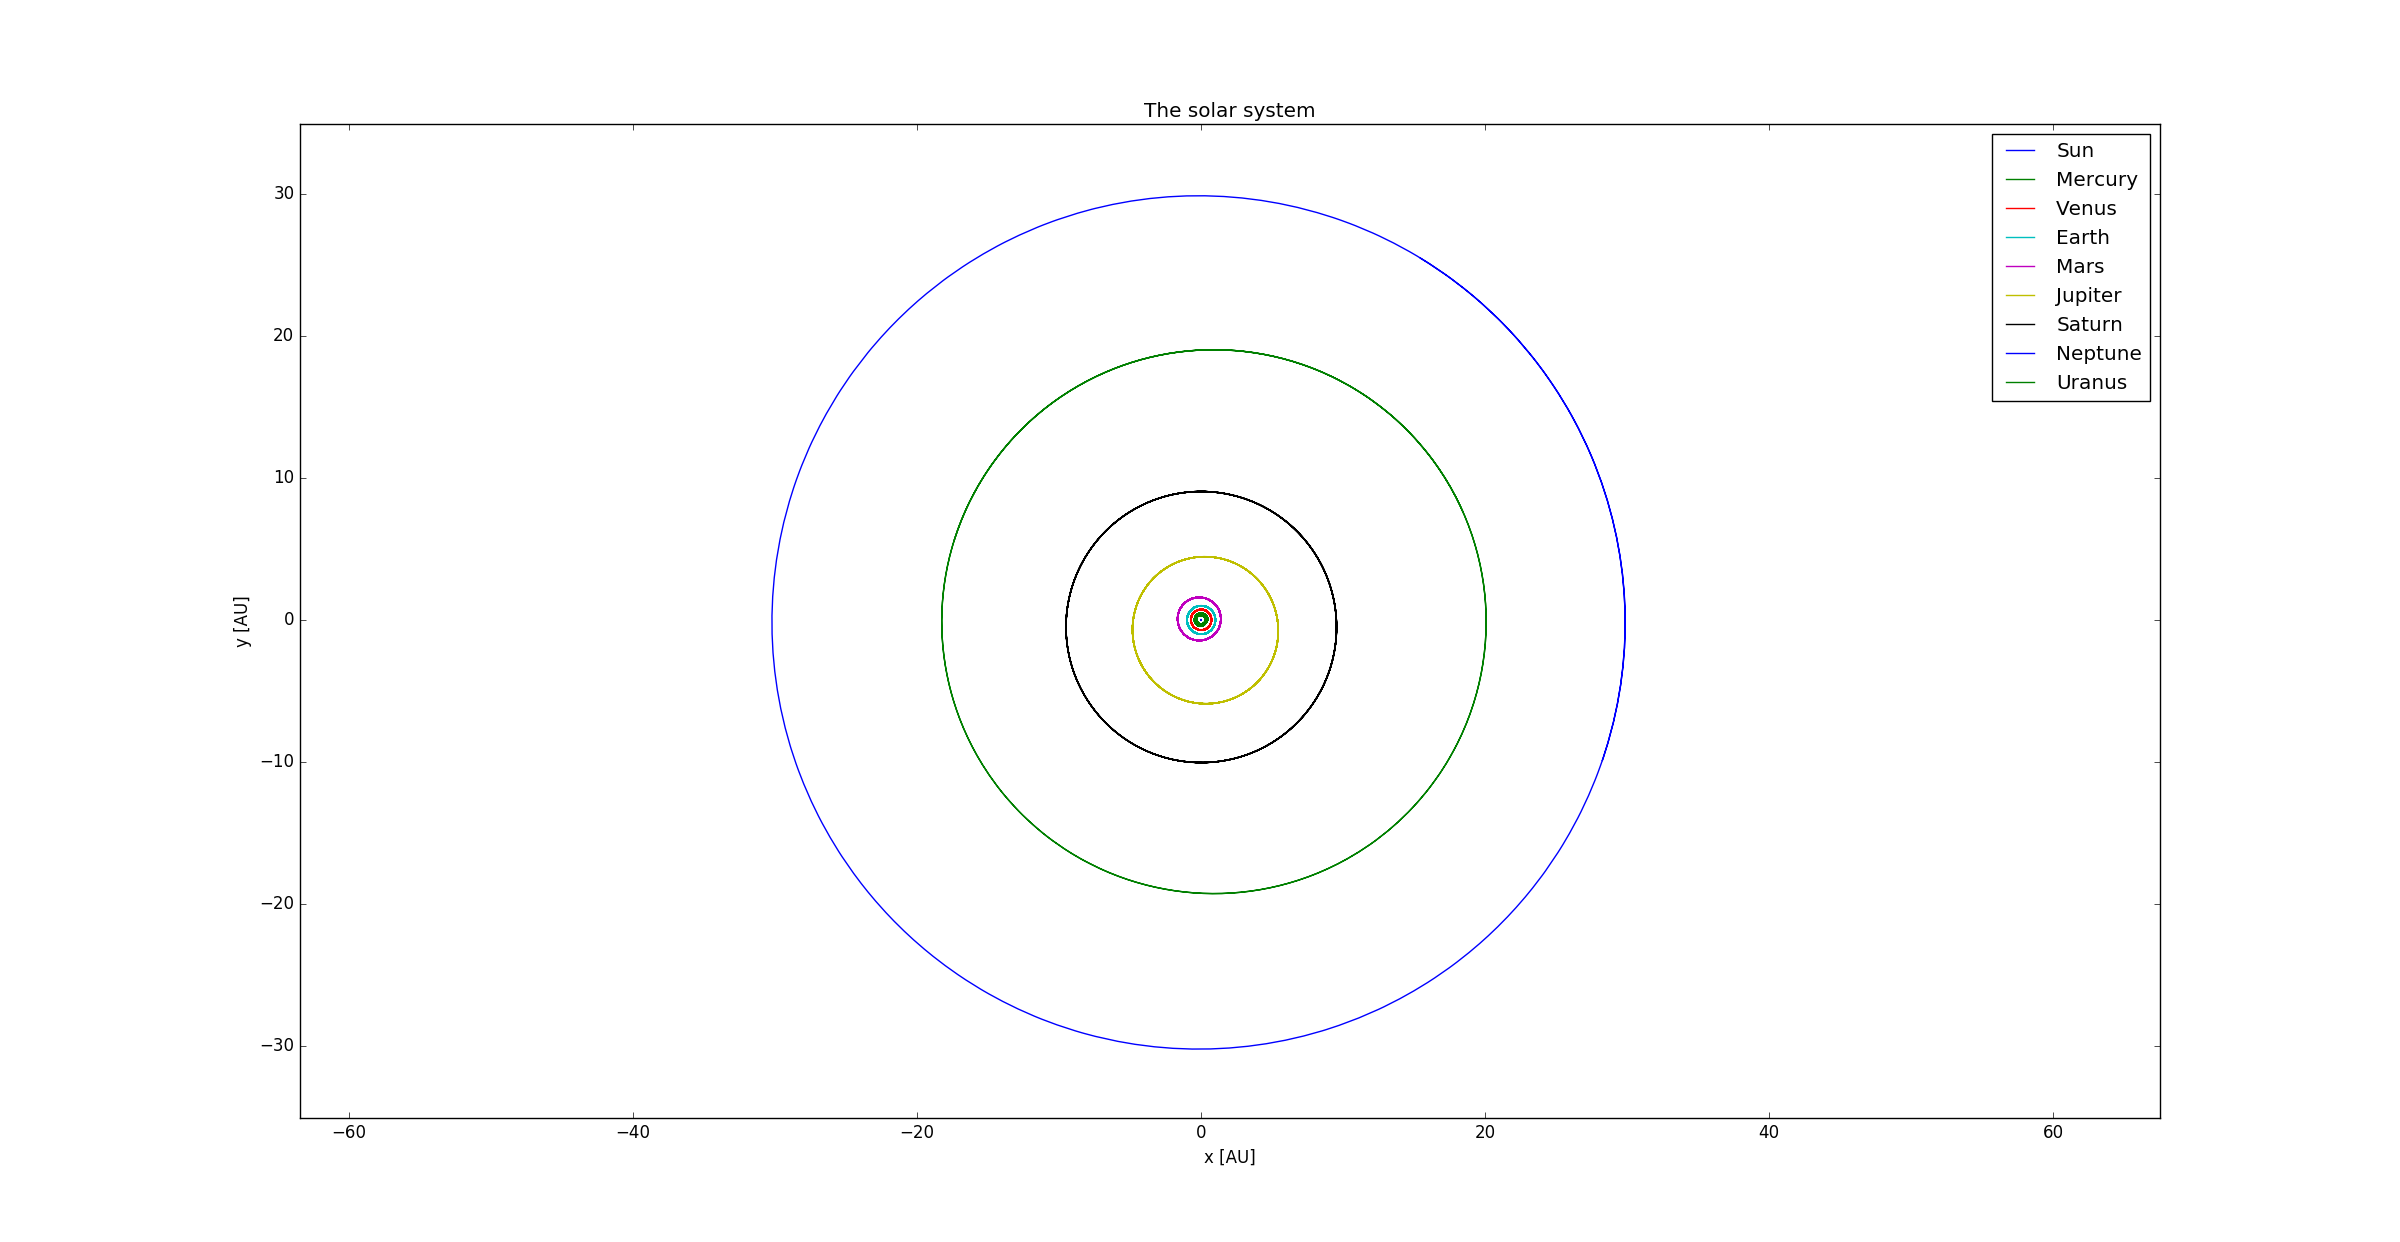
\includegraphics[width=\textwidth]{figures/solarsystem}[h]
\caption{The plot shows the orbit of all the particles in the Solar System around the barycentre}
\end{figure}

